\section{P2P identification schemes}

%% INTRO
 As P2P systems grow in complexity, a way to identify individual users among the
network nodes is needed. To attain this, additional protocols are needed to
ensure that the identity of a node corresponds truthfully to the user it
proclaims to be. A basic way to identify a registered user is by the use of
a private/public encryption scheme. While this can work in simple environments
with a few known users, to allow registration over the network a way to store
the user keys and verify their authenticity is needed.
Next we are going to detail an identification scheme that allows user
registration and identification using the user's username and password.

%% END INTRO

% TODO for revision
The subject of securely establishing stable identities in P2P
systems has been previously studied, for instance, by Aberer,
Datta and Hauswirth~\cite{1318567}. The need for identities mainly arose
from technical concerns, such as handling dynamic IP address
assignment, or avoiding Sybil attacks~\cite{the_sybil_attack}. Authentication of a
node is done via a signature key, automatically generated and
stored on the node.

Traditionally, P2P networks identified the different nodes that compose the
system, but not the user behind each one of them as a different being.
As P2P systems grew in complexity, the need to identify users inside the
network arose.

% TODO for revision
Some P2P storage systems also use techniques which are
related to ours. For example, the DHT-based systems GNUnet
and Freenet use keyword strings to derive a public-private key
pair. The private key is used to sign data and the hash of
the public key to identify the data in storage. Both of
these systems use a keyword string as a seed to a pseudo-random number
generator that produces the key pair~\cite{clarke2010private},~\cite{Bennett03anencoding}.
Knowing only the memorable keyword string the user can
store and retrieve information.

% TODO for revision
Related to forgotten passwords, recovery of information in a
P2P scenario has been studied by Vu et al.~\cite{5380695} who proposed
a combination of threshold-based secret sharing with delegate
selection, and encrypting shares with passwords.
Frykholm and Juels~\cite{Frykholm:2001:EPR:501983.501985} proposed a password-recovery
mechanism based on security questions very similar to our
protocol for the same task. They offer better information-theoretic security properties, something not applicable to our
scenario. We address the subject of password change, which is not applicable to
their scenario, although their proposal could be extended to support password
change using our techniques.

\subsection{Using centralized authorities for the user identification}

\subsubsection{Fully centralized solutions}

Symmetric key cipher-based authentication methods
such as Kerberos~\cite{neuman1994kerberos}, and public key cipher-based
authentication methods such as X.509 (PKI)~\cite{solo2002internet}, are
server-based authentication solutions. In Kerberos, all
users must be registered with the Kerberos server and
the server must share a secret key with each of the participants. The secure channel between each pair of
peers is established on the unique ticket generated by
the Kerberos server, which requires about $O(n^2)$ overhead where n is the total number of members, so the
server easily becomes the system bottleneck. Therefore,
the Kerberos scheme is not a good authentication solution for P2P applications.

\subsubsection{P2P systems using centralized authorities}


Liu et al.~\cite{liu2009efficient} analyzes how to ensure that only
authorized users can access the original media in the P2P live 
streaming system by adopting a user authentication and key management scheme.

The major features of this system include the management server issues each authorized user a
unique public key certificate, the one-way hash chain extends the certificate’s lifetime, the original
media is encrypted by the session key and delivered to the communication group, and the session key is
periodically updated and distributed with the media.

\paragraph{User authentication scheme}
Their user authentication scheme relies in a
authorization server (AS) which issues to each new user a
unique public-key certificate.
The certificate signature is generated from the private
key of the AS and the corresponding public key is published to all the communication group members to verify the certificate presented by any other participant.
The certificate lifetime is based on the media content,
i.e., it is valid during certain frames. 

The AS periodically delivers a certificate revocation list (CRL) to the
participants via a P2P overlay network. Each user receives the CRL by push or
pull transfers with the media distribution. The CRL identifies revoked
certificates for users who have departed but their certificate
 has not yet expired. Since the lifetime is limited, the
CRL needs fewer certificates which reduces the
communication overhead.

While their scheme employs a one-way hash chain to extend the
certificate’s lifetime, which significantly reduces
the computational overhead for the certificate update, the high computational cost
for the re-signature process remains when
an user needs to renovate his certificates from the AS. 

To guarantee that only authorized users can access the
original media even when eavesdropping occurs, their scheme encrypts all the 
original content being delivered in the distributed system.
Using the inmediate neighbors of each node in the P2P system,
their scheme distributes the sessions keys generated by an user with their
authentication scheme.
In this way, a session key is propagated to
all the online users in a hop-by-hop fashion through the network. They rely in their user authentication sheme to establish a secure channel
between peers. 

%% This thing is wrong in so many places
Relying in the underling P2P structure for the sessions keys storage is
not enough to maintain a high availability of them in the network. Depending in
the maitenance for the P2P storage service used there can be times where a
session key can be unavailable to be retrieved. Also, malicious
nodes can still lie about them or refuse to distribute them through the
network. To solve this, reputation schemes can be used to reduce the
probability of failure in the system operations.


Lin et al.~\cite{lin2008p2p} propose to use peer-to-peer (P2P) technology to
establish blog services while using OpenID to provides secure and unified
authentication mechanism. OpenID provides single sign on, multiple accounts and
passwords recovery functionalities. They presents a blog service platform which integrates the P2P networks and the
OpenID authentication mechanism together.



%%\subsubsection{conclusions}


The most important flaw of this type of systems is that a centralized authentication service in a P2P network becomes the system
bottleneck. To let the P2P system maintain its scalability, our following work will focus in a
fully distributed solution for this problem.

%\subsection{Plain PKI scheme}
\subsection{Peerson username/password scheme}

Kreitz et al.~\cite{kreitz2012passwords} present a suite of protocols for password
authentication in P2P networks: account registration, login, password change,
remembered logins, logout from a remote device, and password recovery.
Password authentication is based on standard cryptographic techniques and can
be used with standard P2P components. 

It relies on the safe storage, distribution and retrieval of a a)~\textit{login information
file}, a b)~\textit{device login info file} and a c)~\textit{key store
file}~\ref{fig:p2p_peerson}.

\begin{enumerate}[a)]

  \item The login information file stores encrypted files and a
plain text. The encrypted files are: the user session information (\textit{devmap}), a
cryptographic key for write authentication ($K_W$), and the \textit{filename of the
key store file} ($f_{KS}$) along with the \textit{symmetric key} used to encrypt and
decrypt the \textit{key store file} ($K_{KS}$). The plain text is a random byte string used as a \textit{salt} to generate the user private key to
decrypt the first bundle of files. 

  \item The \textit{key store file} ($F_{KS}$) stores all the private keys used to identify the
    user in the system services. This file is encrypted by the $K_{KS}$ key.

  \item The device login information file only stores the filename of the key
    store file and the $K_{KS}$ key, both of which are encrypted by a $K_{DL}$ key
    stored in the \textit{devmap}.
\end{enumerate}

\begin{figure}
\center
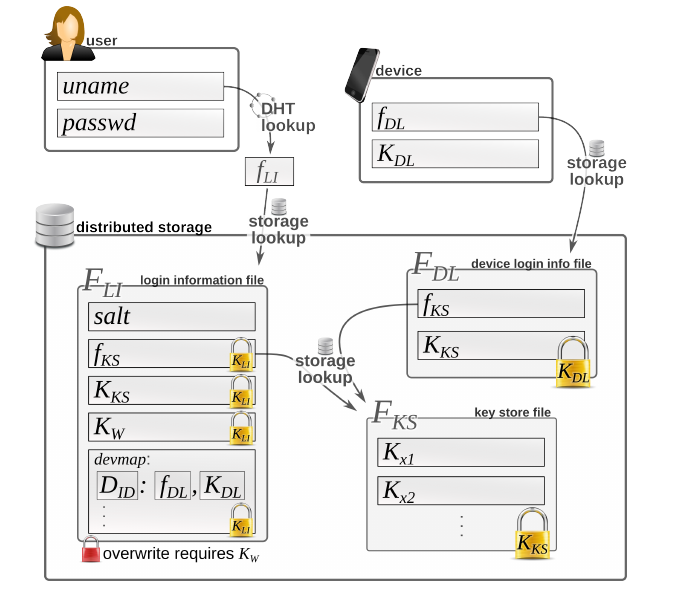
\includegraphics[width=12cm]{../img/password_peerson}\\
\caption{Peerson scheme storage locations (boxes) and login procedure (arrows) }
\label{fig:p2p_peerson}
\end{figure}

Their protocols are as follows:
%
%% introduction of identification schemes. Par 2: proposed username/password identification schemes. Part 3: securing the network protocols. Part 4: Pending issues.
\subsubsection{Account registration}
%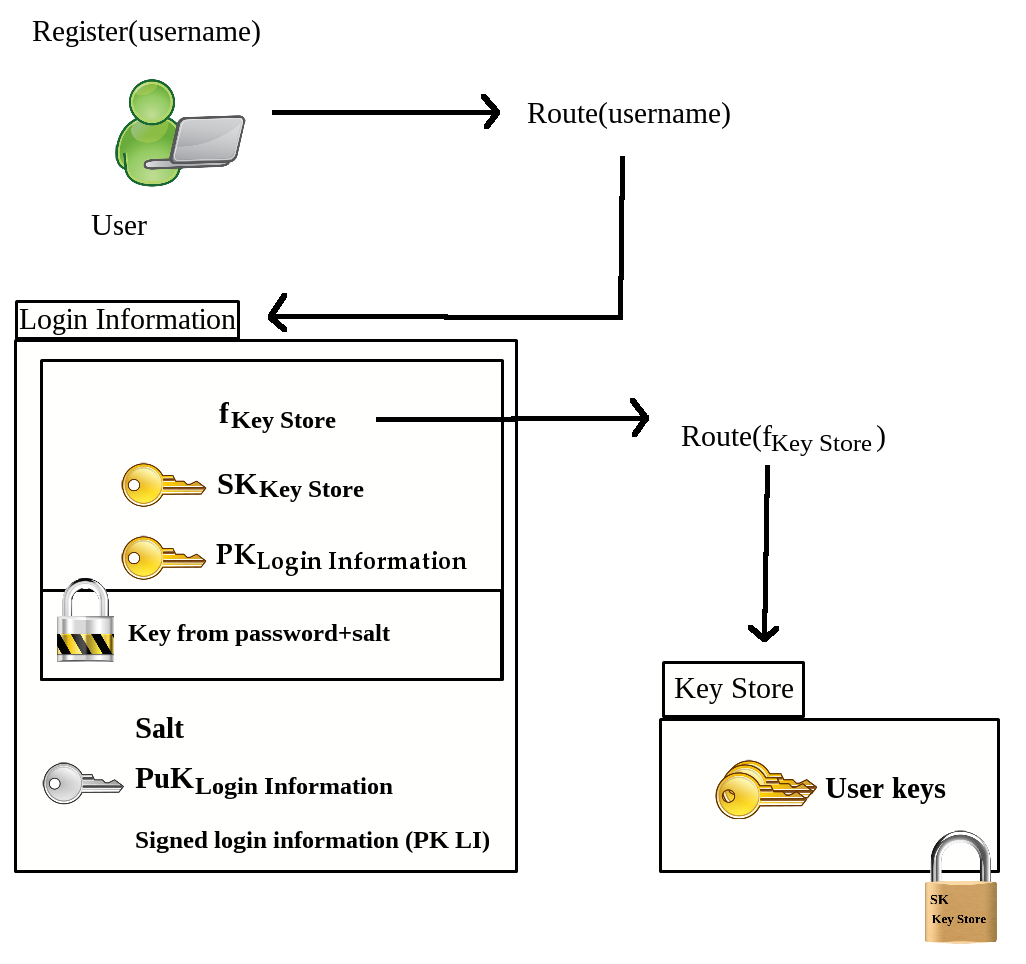
\includegraphics[width=14cm]{../img/user_registration}\\

To register a new user account, the user first
has to choose a \textit{username} and a \textit{password}.
In the key-based authentication, the user creates a \textit{key store
file} $F_{KS}$, containing all the
keys used by the P2P application the user wants to login to.
The user generates a cryptographic key to authenticate the write operations
that will be made in the file. The cryptographic key is then stored with the
other keys in the \textit{key store file} $F_{KS}$.

% encryption and store of the key store file
The user then creates a \textit{symmetric key} $K_{KS}$, which is used to
encrypt the file content. Then the ciphertext
is put into storage, obtaining a \textit{filename} $f_{KS}$ for it. Now, the user
creates a \textit{login information file} $F_{LI}$ by creating a random
byte string, or \textit{salt}, and deriving a \textit{symmetric key} $K_{LI}$ from the user
\textit{password} and the \textit{salt}.
Using the new \textit{ symmetric key} $K_{LI}$, the user encrypts the
filename $f_{KS}$,
the \textit{symmetric key} $K_{KS}$ and the cryptographic key to
authenticate the write operations $K_W$.
 The \textit{salt} and the three encrypted values are put
into storage, obtaining a filename $f_{LI}$ . The \textit{salt} is stored
in plaintext, so that the user can later derive the decryption
key $K_{LI}$ by only providing the password. Finally, the user
performs the write-once operation \textit{put} on the DHT, with
username as key and $f_{LI}$ as value.

%unique username
If the username was taken,
the user is prompted for a new username.

%finish
Once all operations
have succeeded, the user is registered in the system.


\subsubsection{login}


The user uses his username to find and retrieve his \textit{login information
file} $F_{LI}$. Then, using his \textit{password} and the \textit{salt} included in the
\textit{login information file} $F_{LI}$, obtains the filename
$f_{KS}$ used to
route back to where the \textit{key store file} $F_{KS}$ is stored.  Lastly, he uses the
\textit{symmetric key} $K_{KS}$ to decrypt the \textit{key store file}
$F_{KS}$ and recover his user keys.

\subsubsection{Password change}
%To change the password, the user has to rewrite his \textit{login information
%file}.


Before the user can change his password, he must login using his password to
obtain the $K_{LI}$ . With this information, the password change can be
completed. The user is asked for a new password and a new \textit{salt} is
generated. The key-derivation function is used to generate a new key
$K_{LI}^{new}$
for the login information file. Then, the content of the \textit{key-store
file} is
retrieved and decrypted (with the old key). A new key $K_{KS}^{new}$ is generated and
used for encrypting the key-store content again before it is saved in the
storage system. The storage of the key-store content returns a new filename $f_{KS}^{new}$.
Finally, the \textit{login information file}
is updated: $f_{KS}^{new}$, $K_{KS}^{new}$, the write credential $K_{W}$ as well as a new empty
device mapping file \textit{devmapnew} are encrypted with the new key $K_{LI}^{new}$.
  Together with the new \textit{salt}, this ciphertext is written to the distributed
storage, using the reference $f_{LI}$ and the credential $K_W$, to authenticate the
write operation. Lastly, the keys stored in the key-store should be updated by
the application using the P2P protocol.  At this point, old device login
information files can also be deleted from the
storage to reclaim space.

\subsubsection{Logout}
%The system does not have something like a "session" to maintain; the only way
%to identify an user is by his keys that are obtained by the identification
%process.

To logout from the system, the user does not have to interact
with the DHT or the storage system. Simply wiping the local
cache from application data and all key material restores the
pre-login state. If the user chose to remember the login on a
device, the corresponding \textit{device login information file} $F_{DL}$
can also be deleted from storage.
 A problem related to logging out is revoking remembered
credentials on another device, e. g., a user’s stolen phone. To
accomplish this, they first run the password change operation,
which locks out all devices with remembered logins, because
the key store key $K_{KS}$ changed (as well as the filename $f_{KS}$).
Next, we use the device mapping file \textit{devmap} to inform all devices
about the new key (and filename), except the device that is to
be revoked. To inform a device about the change, we update
the corresponding values in the device’s \textit{login information file}
 $F_{DL}$ which can be accessed from the device by using the
locally stored credentials.

 After running the password change
operation, all devices that should not be revoked and that have remembered
logins (and therefore are referenced in the \textit{devmap}) are
processed. The \textit{device login information filename} $f_{DL}$ and its key $K_{DL}$ are read,
and the new key store key $K_{KS}^{new}$ and filename $f_{KS}^{new}$ are written to the
\textit{device login information file} $F_{DL}$, encrypted under the device key $K_{DL}$.
Finally, the modified \textit{devmap} is saved back to the \textit{login
information file} $F_{LI}$.


\subsubsection{Forgotten passwords and password-recovery mechanisms}
  %- HUGE danger
  %- Security questions
  %- threshold-based secret sharing with delegate selection and encrypting
  %shares with passwords

%%%%%%%%%%%%%   Peerson Passwords in P2P networks %%%%%%%%%%%%%
%An important part of password-based logins is the possi-
% bility for users to recover their accounts if they forget their
% passwords. We refer to this as a password recovery mechanism.
% The goal of a password recovery mechanism is to provide a
% secondary way of authenticating the user. There are a number
% of password recovery mechanisms used in practice. In our
% experience, three of the most common ones are password
% hints, security questions, and e-mail based recovery. Other
%
%approaches (beyond the scope of this paper) include vouching
%for identity by social contacts [21], or using trusted devices.
% Password hints means that the user may enter a hint at
%the same time as she sets this password. The hint will be
%displayed to her if she forgets her password, and should be
%selected such that it helps her recall her password, but does
%not make it significantly easier for someone else to guess it.
%The hint is not truly a secondary authentication mechanism,
%but rather a means to recovering the original password-based
%authentication mechanism. A basic version of password hints
%would be straightforward to implement in our system: the
%hint can be stored in plaintext in the login information file.
%Security questions and e-mail based password recovery are
%more complex to adapt. We described their implementation in
%detail after listing requirements.
%
% As in Section IV for the login procedure, we define a set of
%functional requirements for password recovery, based on the
%ISO 27002 standard [19] as follows. We also augment the list
%with requirements of our own (preceded by a star).
%establish methods to verify the identity of a user prior to
%•allowing the user to choose a new password
%communicate with those affected by or involved with
% - recovery security incidents
% - have procedures to allow recovery and restoration of
%business operations and availability of information in a
% time-scaled manner
%a legitimate user should be able to recover lost (forgotten)
% - or broken (device’s) keys
% - the recovery procedure should allow a user to set a new
% password, not reveal the old password
% - the process of recovery should be easy to use
% - sensitive information for recovery should be kept secret
%
%Our protocols support these requirements.

%% The sole exception
%% is that if a password is reset via security questions alone, the
%% system would not “communicate with those affected” (e.g.,
%% send an e-mail notification that the password had been reset,
%% as is common in centralized services). We remark that the
%% last item is a property many centralizedstronger than systems
%% provide. In our system, no one learns the answers to a user’s
%% security questions. We consider this to be important, since
%% many systems use similar security questions.
%% 
%%  The operations described in this section imply minor addi-
%% tions to the protocols of Section IV, i. e., invoking the update
%% procedures after each password change (to sustain transaction
%% safety, the updates have to be included in the final write
%% operation of the password change operation).
%% A. Security Questions
%%  Security questions is a password recovery technique that
%% relies on answers to questions the user is asked during regis-
%% tration. The answers should be such that they cannot be easily
%% guessed or researched by an attacker, but still stable over
%% time, memorable, and definite [22]. Rabkin [23] underlines
%% the importance to choose good questions especially in the era
%% of social networks. Frykholm and Juels [12] discuss a related
%% technique that is similar to our adaption of this scheme.
%% %%%%%%%%%%%%%   Peerson Passwords in P2P networks %%%%%%%%%%%%%

Depending on the desired functionality of the network, they propose two
mechanisms to provide user password recovery. The actual implementation
requires small modifications in the protocols seen above.

\paragraph{Using security questions.}

 The protocol assume that the user provides $n$ answers $A_i$ to suitable
 security questions $Q_i$ . In order to recover the password, it is
 required for the user to answer any $k$ out of these $n$ questions
 correctly. The choice of $k$ constitutes an obvious trade-off
 between security and usability. A successful recovery yields
 the key $K_{LI}$ to the login information file, allowing the user to
change the password. The implementation
does not require the user to provide new answers after a regular
 password change. Additionally, the protocol avoids storing the plaintext
 answers to the security questions.
 For the setup of the question based recovery mechanism, the protocol first
create $n$ shares $qS_1, \cdots, qS_n$ of the
 key $K_{LI}$ under an $(n, k)$-secret sharing scheme. For each of
 these shares, it is created a salt $qsalt_i$ , derived a key $qK_i$ from
 this salt and the answer $A_i$, and used it to encrypt the share,
 yielding $qS^{enc}_i$. Furthermore, it is encrypted the key $qK_i$ with
 the login information file key $K_{LI}$, for the update procedure
 described later. Finally, the login information file is extended
 with all questions $Q_i$, the salts $qsalt_i$, the encrypted shares
 $qS_i^{enc}$ and the encrypted keys $qK_i^{enc}$. When recovering, the
 user has to reproduce at least $k$ answers, which together with
 the stored salts can be used to derive $k$ keys $qK_i$, which in
 turn can decrypt $k$ shares $qS_i$.
 When $K_{LI}$ changes (e. g., due to a regular password
 change), we update the recovery information %as in~\ref{sec:}
 for the new key $K_{LI}^{new}$, a new set of shares is created.
 Next, the keys $qK_i$ are decrypted and used to encrypt the new
 shares. Neither the keys $qK_i$ nor the salts $salt_i$ change, so
 the user can still use the same answers for recovery. Finally,
 the updated shares (and re-encrypted keys, to allow further
 updates) are saved back to the login information file.

\paragraph{Email based.}

  In e-mail based password recovery, the user is sent an e-mail
 containing some information, typically a link with a token, by
 which she can reset her password. This link is sent to an e-mail
 address she has registered with her account.
 We adapt this scheme by randomly choosing a number of
 peers, that collaboratively provide this functionality to the user.
 

 It use $(n, k)$-secret sharing to enable password recovery even
 if not all of the involved peers are online when the user wants
 to recover the password.
 To provide persistence of the recovery mechanism independent of a changing key $K_{LI}$ (e. g., due to a password change),
 the result of the recovery process is a recovery key $K_R$ ,
 that always encrypts the current version of $K_{LI}$.
  From the recovery key $K_R$, $n$
 shares $eS_1, \cdots, eS_n$ are generated using $(n, k)$-secret sharing.
 For each share, a random peer $peer_i$ is picked, two salts $esalt_i$
 and $ksalt_i$ are created and a cryptographic commitment $C_i$ is
 derived from the salt $esalt_i$ together with the email. This
 commitment will be used to authorize the user to the peer,
 and bind it to this specific e-mail address. Next, a key $eK_i$,
 to encrypt the share $eS_i$ , is derived in the same way as the
 commitment, but with salt $ksalt_i$. A different salt is needed
 so that the peer cannot decrypt the share (before learning the
 address). The commitment and the encrypted share are stored
 at the peer. The login information $F_{LI}$ file is extended with a
 list of the chosen peers $peer_i$ and the according salts $esalt_i$ ,
 $ksalt_i$, as well as $K_{LI}^{enc}$, encrypted with the recovery key, and
 the recovery key, encrypted with $K_{LI}$ (to allow for password
 changes).

 To recover the password, the user looks up the
 available information in the login information file, including
 the list of peers to be requested for assistance. Each request is
 authorized by the commitment $C_i$, that the peer can derive
 from the salt $esalt_i$ and the e-mail address that the user
 provided. If the request was legitimate, the peer
 sends the encrypted share to the e-mail address. As soon as
 the user collected $k$ answers, he can recover $K_{LI}$ .

 To provide long-term persistence of this recovery mechanism, $K_{LI}^{enc}$
 has to be updated whenever $K_{LI}$ changes.
 
 \paragraph{Combining Approaches}
 Also mentions a combining approach using questions and email recovery, either
sequentially or in parallel.
  By sequential composition, they mean
 that the user must both correctly answer security questions and
 receive e-mail. In parallel composition, either
 mechanism can be used alone to recover the password. The
 latter is achieved by using both systems in parallel.
 For sequential composition, the user picks a uniformly
 random string $r$ of the same length as $K_{LI}$. The user stores $r$ in
one of the mechanisms, and $K_{LI} \bigoplus r$ in the second mechanism, where
$\bigoplus $ denotes the exclusive-OR operation.

  If one recovers both of these, $K_{LI}$ can be computed. If one learns only one
 of the pieces, nothing is gained, as both $r$ and $K_{LI} \bigoplus r$ are
 uniformly random. More generally, to combine $n$ mechanisms
  in arbitrary ways, $(n, k)$-secret sharing can be used. What they
 describe there are two trivial such schemes for $n = 2$.\\



%\section{Keys generation}
%\subsection{Randomly derived}
%  manual backup of the keys
%\subsection{Keys derived from a password}


\subsubsection{Conclusions about Peerson proposal}

Their proposal describes what is needed to obtain a P2P username/password based
identification system, but they do not go deeper beyond that. They are problems
that are not 

% TODO: IDEAS SPANISH
%====== IDEAS IN PROGRESS ======
%
%Un problema importante es que su systema de identificacion falla en la
%precencia de nodos maliciosos. Esto es debido a que carece de un sistema que
%discrimine a los nodos segun su comportamiento, haciendo que bajo una cantidad
%baja de nodos maliciosos el sistema tenga altas probabilidades de falla. A
%pesar de que nombran el problema, no proponen soluciones que realmente
%solucionen el problema.
% %Por ejemplo, si consideramos el registro de usuarios  
%
%Ademas, considerando que ellos asumen que los tiempos de lectura y de escritura
%de la red de almacenamiento distribuida son iguales a los de la consulta por
%una llave específica en un DHT.
%
%====== IDEAS IN PROGRESS ======

The problem with the existing protocols is that they do not implement measures against the presence of malicious nodes.
A malicious or byzantine node is any node that does
not behave as expected by the protocol of the system. The presence of this type
of nodes can easily break the security and degenerate the quality of the
service in the whole system.
